\documentclass{article}
\usepackage[T1]{fontenc}
\usepackage{titlesec}
\usepackage{graphicx}
\usepackage{amsmath}
\usepackage{xcolor}
\usepackage{amssymb}
\usepackage{circuitikz}
\titleformat{\section}  % which section command to format
  {\fontsize{10}{12}\bfseries} % format for whole line
  {\thesection} % how to show number
  {1em} % space between number and text
  {} % formatting for just the text
  [] % formatting for after the text
\title{Logika Cyfrowa}
\author{Jakub Gałaszewski} 
\begin{document}
\maketitle
\section{Pokaż, jak zaimplementować funkcję $f (x, y, z) = \sum m(0, 2, 3, 4, 5, 7)$ przy użyciu dekodera 3 do 8 oraz bramki OR.}
\textbf{dekoder} to zbiór bramek logicznych, które konwertują liczbę w one hot.  
\begin{center}
	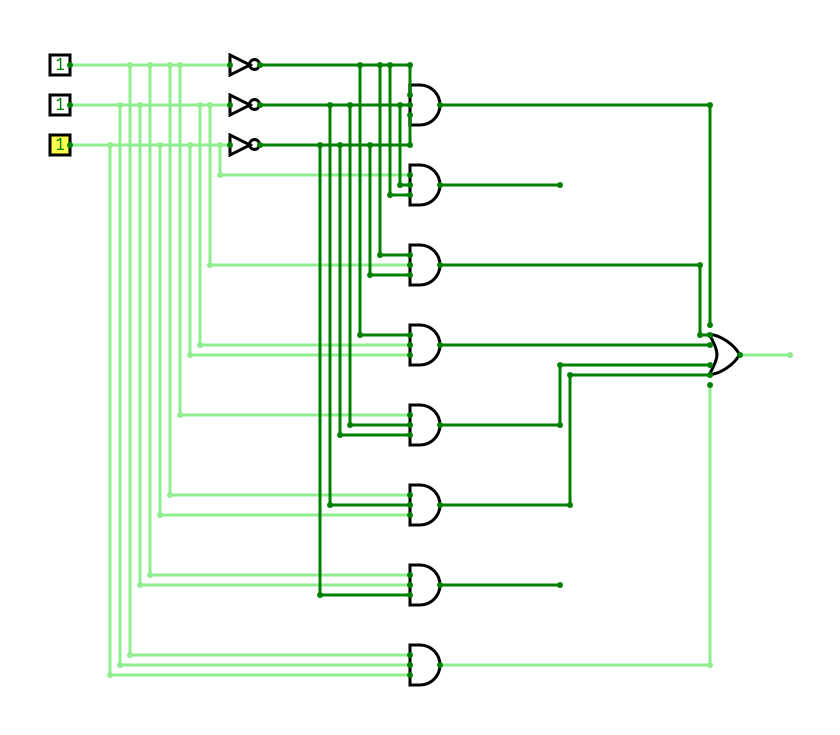
\includegraphics[scale=0.3]{./L04_Z01.png}
\end{center}
\section{Wykorzystaj tabelki logiczne, aby skonstruować obwód wykorzystujący multiplekser dwuwejściowy, który implementuje funkcję $f(x, y, z) = \bar y\bar z + xy$.}
\textbf{multiplekser} to taki układ cyfrowy, gdzie jedno wejście decyduje o tym jakie wyjście chcemy zwrócić.
\begin{center}

\begin{tabular}{|c|c|c||c|} 
	 \hline
	$x$ & $y$ & $z$ & $\bar y\bar z + xy$\\ 
	 \hline \hline
	 0&0&0&1\\ \hline
	 0&0&1&0\\ \hline
	 0&1&0&0\\ \hline
	 0&1&1&0\\ \hline
	 1&0&0&1\\ \hline	 
	 1&0&1&0\\ \hline
	 1&1&0&1\\ \hline
	 1&1&1&1\\ \hline
\end{tabular}\\
	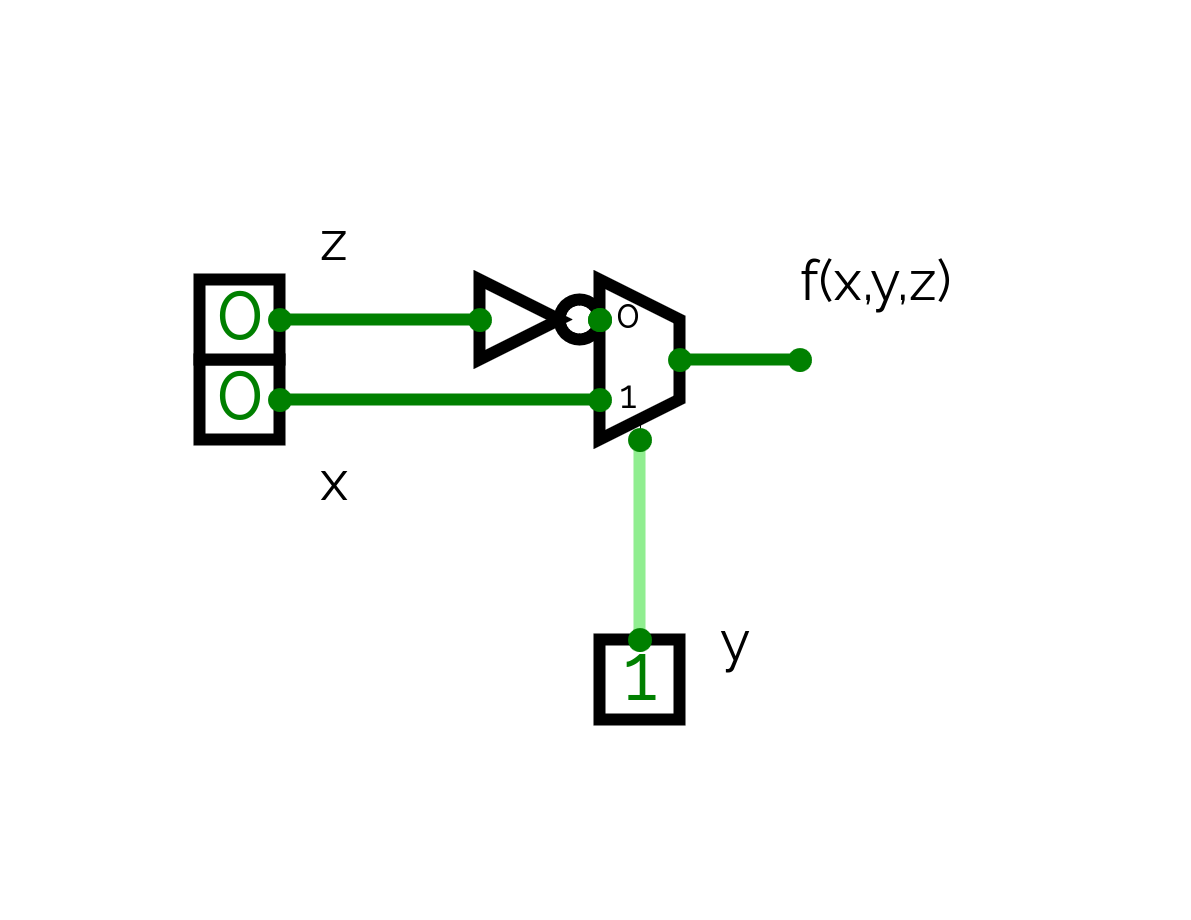
\includegraphics[scale=0.2]{./L04_Z02.png}
\end{center}
\section{Wykorzystaj rozwinięcie Shannona, aby skonstruować układ implementujący funkcję $f(x, y, z) = \sum m(0, 4, 6, 7)$ wykorzystujący multiplekser dwuwejściowy i ewentualne bramki pomocnicze.}
$f(x, y, z) = \sum m(0, 4, 6, 7) = \bar{x}\bar{y}\bar{z} + x\bar{y}\bar{z} + xy\bar{z} + xyz$\\
$f(x, y, z) = \sum m(0, 4, 6, 7) = x f(1,y,z) + \bar{x}f(0,y,z) = xyf(1,1,z) + x\bar yf(1,0,z) + \bar xyf(0,1,z) + \bar x\bar yf(0,0,z)$
\begin{center}
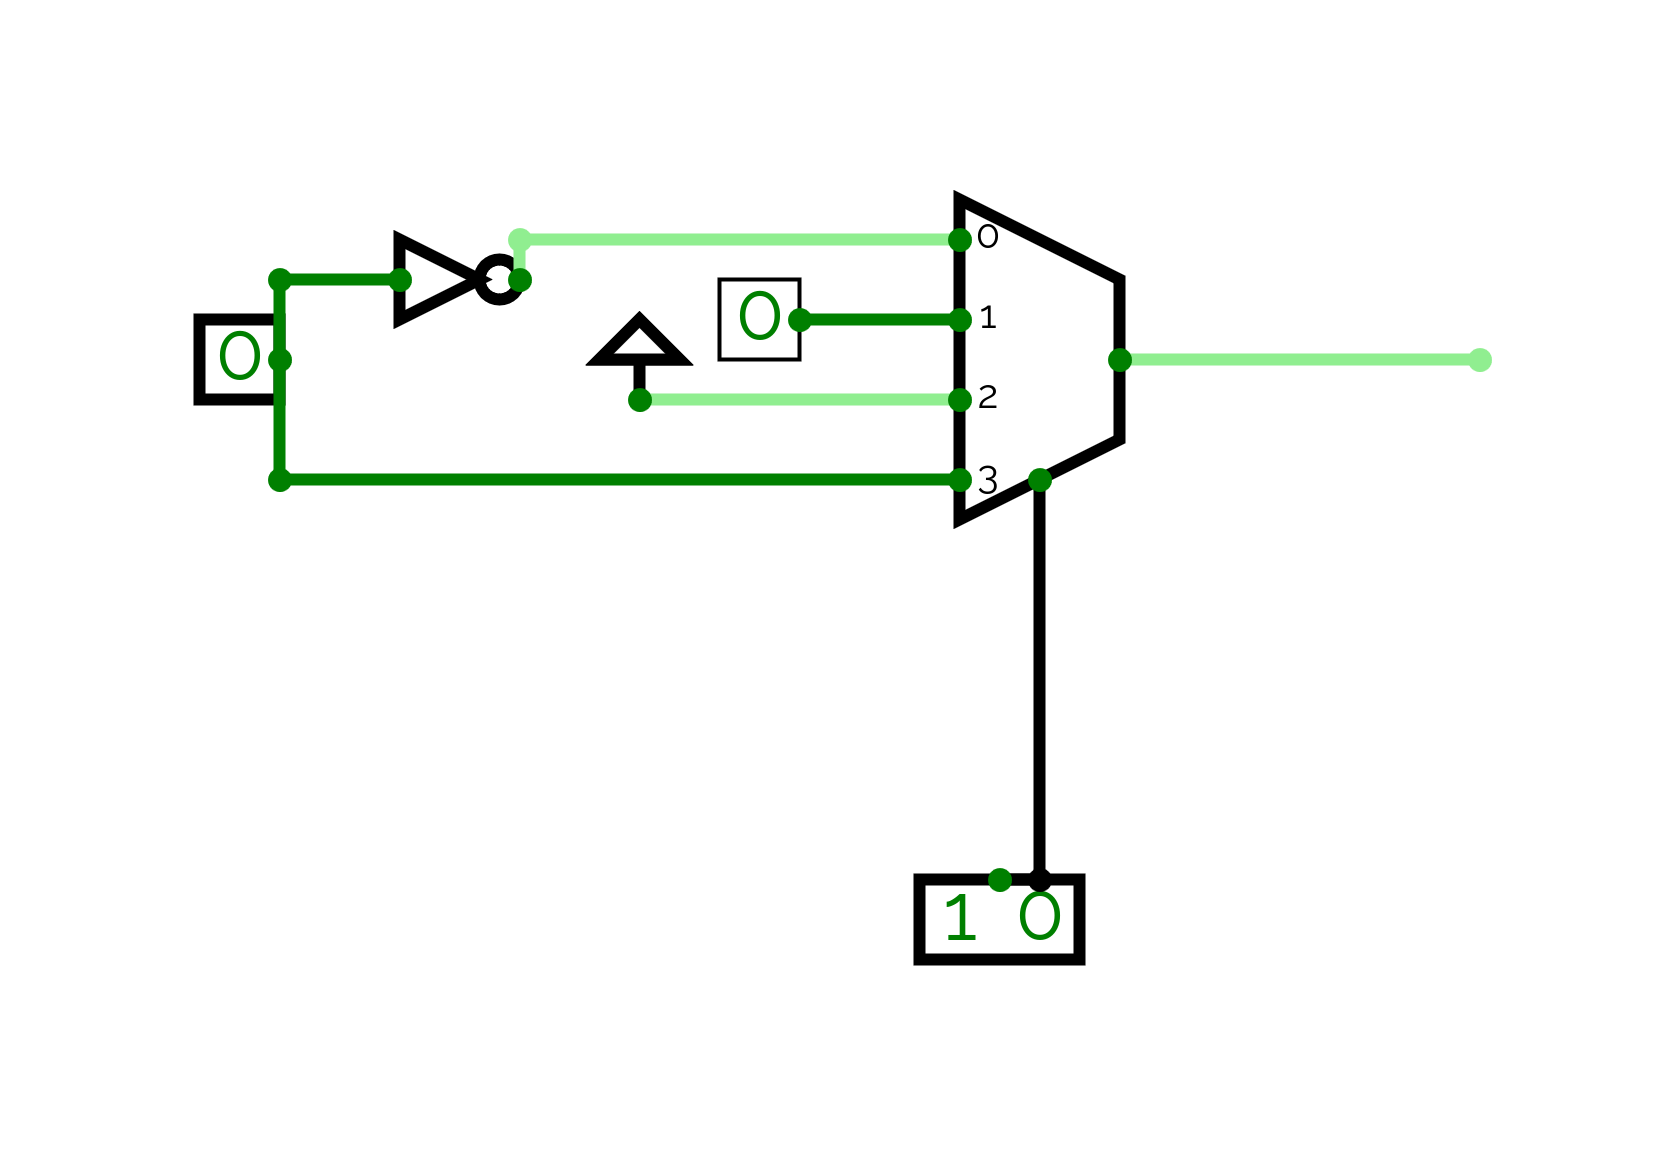
\includegraphics[scale=0.2]{./L04_Z03.png}
\end{center}
błąd, prosili nas w zadaniu o multiplekser dwuwejściowy.
\begin{center}
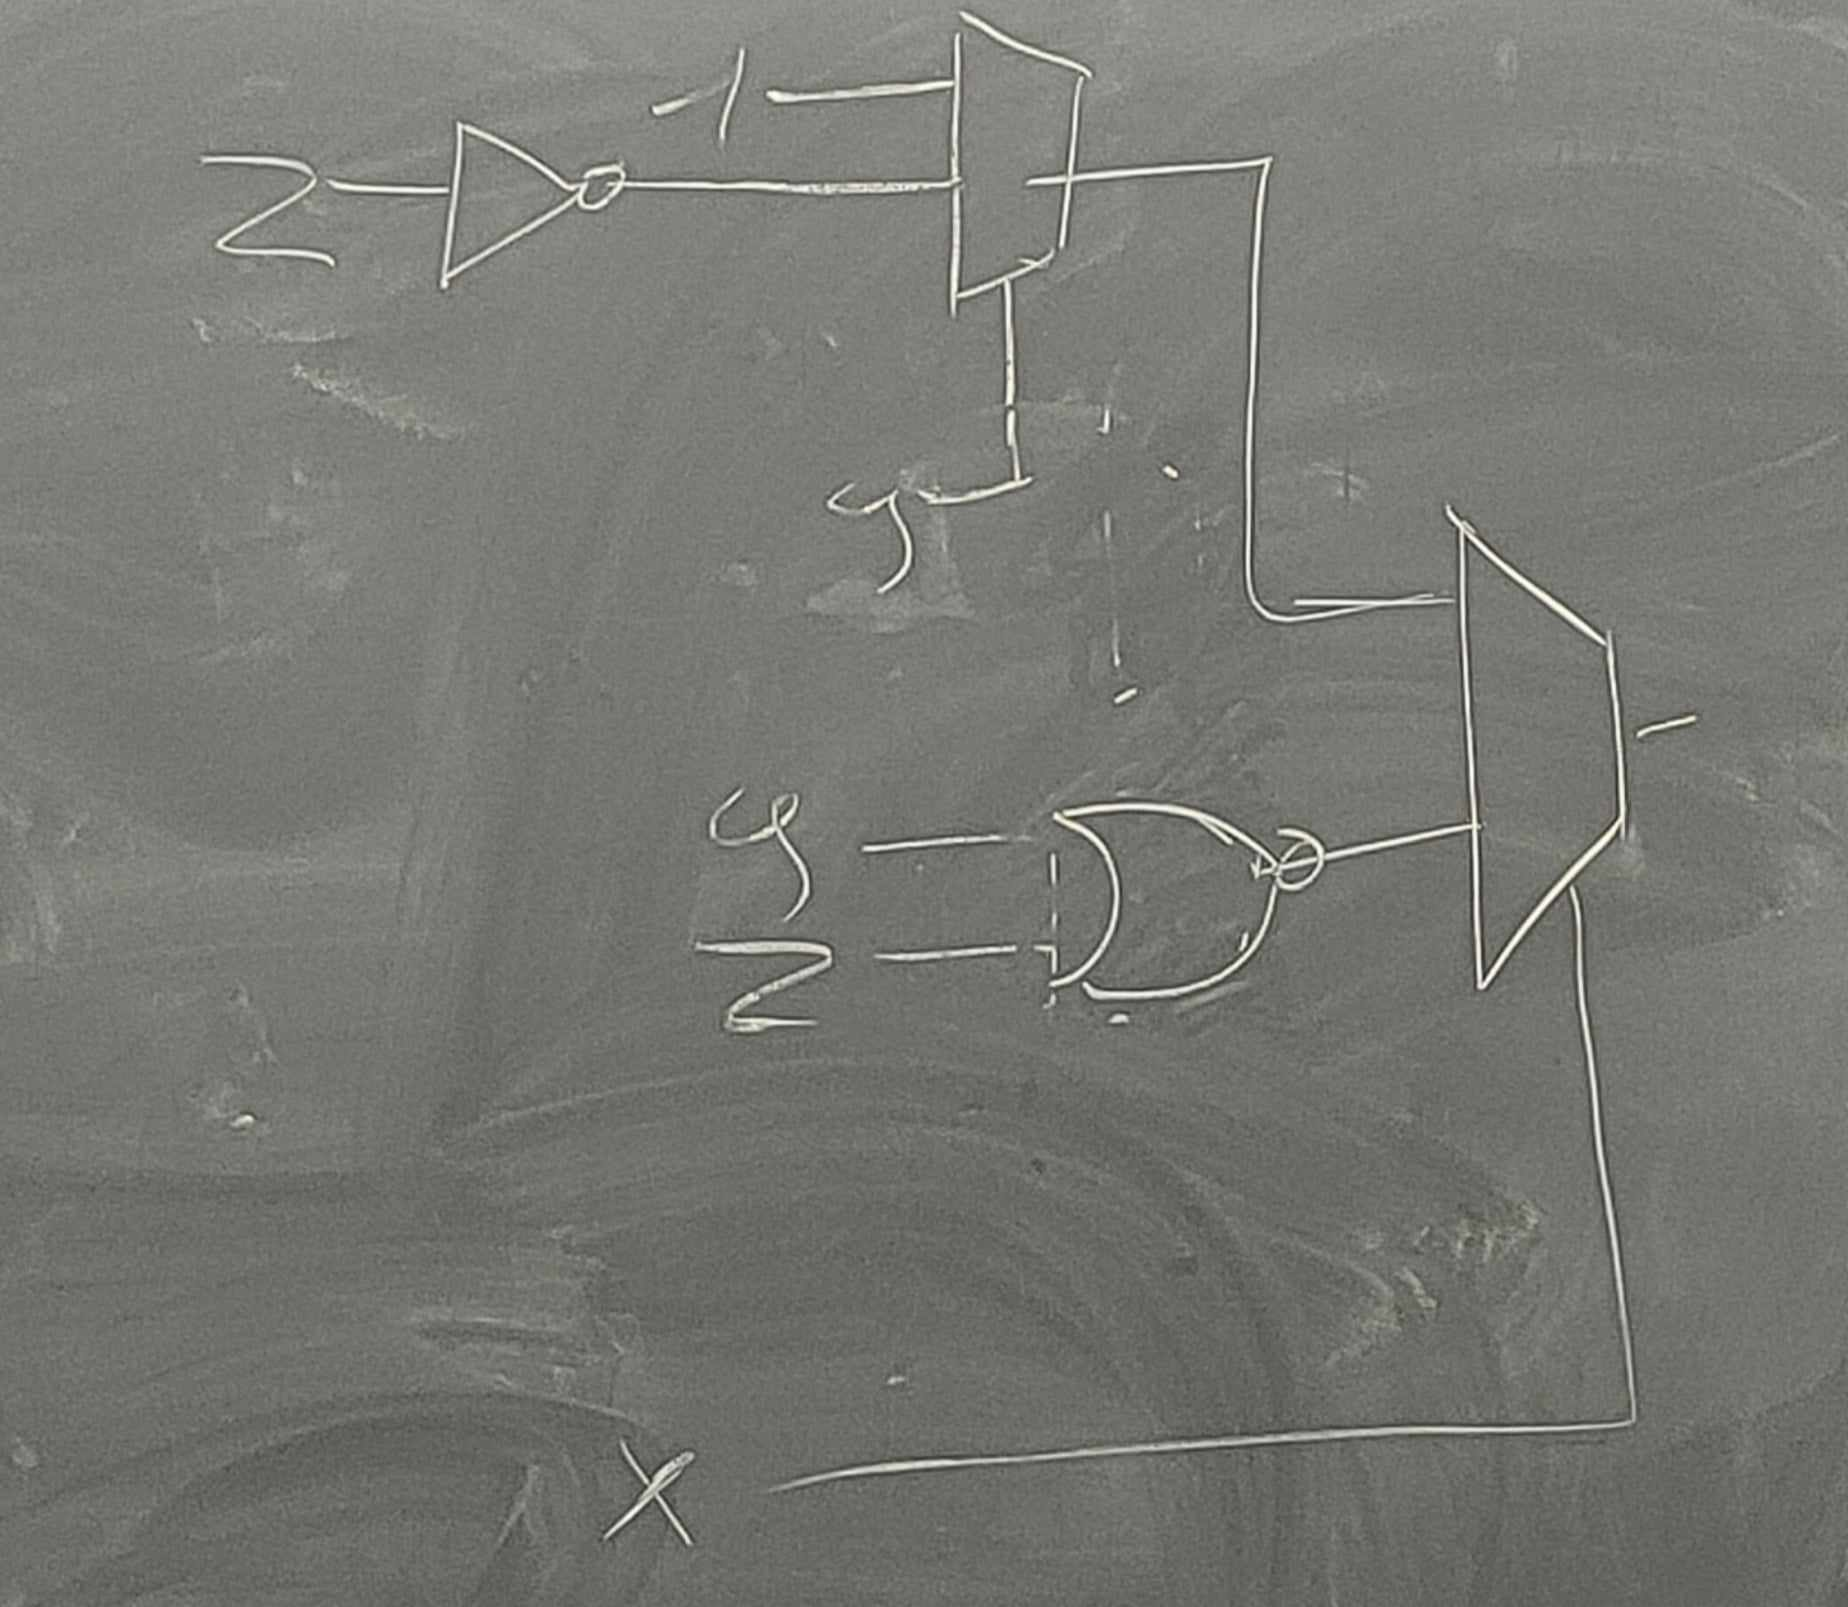
\includegraphics[scale=0.2]{./L04_Z03II.jpg}
\end{center}
\section{Pokaż, jak wylistować wszystkie mintermy funkcji $f(x, y, z) = \bar y + \bar x \bar z + xz$ używając rozwinięcia Shannona}
$f(x, y, z) = \bar y + \bar x \bar z + xz = xf(1, y, z) + \bar{x}f(0, y, z)= x(yf(1, 1, z) + \bar{y}f(1,0,z)) + \bar{x}(yf(0, 1, z) + \bar{y}f(0,0,z)) = x(y(zf(1, 1, 1) + \bar{z}f(1,1,0) )+ \bar{y}(zf(1,0,1) + \bar zf(1,0,0))) + \bar x(y(zf(0, 1, 1) + \bar{z}f(0,1,0) + \bar{y}(zf(0,0,1) + \bar zf(0,0,0))) = xyz + xy\bar{z} + x\bar{y}z  +x\bar{y}\bar{z} + \bar xyz + \bar xy\bar{z} + \bar x\bar{y}z  +\bar x\bar{y}\bar{z}$
\section{Udowodnij twierdzenie o rozwinięciu Shannona (w dowolnej z dwóch dualnych wersji).}
$\Phi = x \wedge \Phi[x/1] \vee \neg x \wedge \Phi[x/0]$\\
rozpatrujemy dwa przypadki:\\
dla x = 1, $\Phi = 1 \wedge \Phi[x/1] \vee \neg 1 \wedge \Phi[x/0] = \Phi[x/1]$\\
dla x = 0, $\Phi = 0 \wedge \Phi[x/1] \vee \neg 0 \wedge \Phi[x/0] = \Phi[x/0]$
\section{Układ przesuwający to układ implementujący funkcję $f (a_{N -1:0}, k_{M -1:0}) = a_{N -1:0} \ll k_{M -1:0}$ (lub analogiczną, dla operatorów $\gg, \lll, \ggg $). Pokaż, jak skonstruować układ przesuwający używając tylko $N log_2N$ multiplekserów dwuwejściowych.}
TODO
\section{Napisz minimalne wyrażenia w DNF dla wyjść d, e, f , g dekodera dla wyświetlaczy 7-segmentowych.}
"Zapożyczone" od zeszłotygodniowego Kuby:
\begin{center}
\begin{tabular}{|c|c|c|c|c|} 
	 \hline
	AB\textbackslash CD& 00 & 01 & 11 & 10\\  \hline
	 				 00&1&0&1&1\\ \hline
	 				 01&0&1&0&1\\ \hline
	 				 11&X&X&X&X\\ \hline
	 				 10&1&1&X&X\\ \hline

	\end{tabular}\\
	$$d = \bar{B} \bar{D} + \bar{B}C + B\bar{C}D + C\bar{D} + A$$
	\begin{tabular}{|c|c|c|c|c|} 
	 \hline
	AB\textbackslash CD& 00 & 01 & 11 & 10\\  \hline
	 				 00&1&0&0&1\\ \hline
	 				 01&0&0&0&1\\ \hline
	 				 11&X&X&X&X\\ \hline
	 				 10&1&0&X&X\\ \hline
	
	\end{tabular}\\
	$$ e = \bar{B}\bar{D} + C \bar{D}$$
	\begin{tabular}{|c|c|c|c|c|} 
	 \hline
	AB\textbackslash CD& 00 & 01 & 11 & 10\\  \hline
	 				 00&1&0&0&0\\ \hline
	 				 01&1&1&0&1\\ \hline
	 				 11&X&X&X&X\\ \hline
	 				 10&1&1&X&X\\ \hline
	
	\end{tabular}\\	
	$$f = \bar{C}\bar{D} + B \bar{C} + B\bar{D} + A$$	
	\begin{tabular}{|c|c|c|c|c|} 
	 \hline
	AB\textbackslash CD& 00 & 01 & 11 & 10\\  \hline
	 				 00&0&0&1&1\\ \hline
	 				 01&1&1&0&1\\ \hline
	 				 11&X&X&X&X\\ \hline
	 				 10&1&1&X&X\\ \hline
	\end{tabular}\\
	$$g = \bar{B}C + B\bar{C} + A + B\bar{D}$$
\end{center}
\section{Pokaż, jak zaimplementować funkcję $f (x, y, z) = y\bar z + xz + \bar yz$ używając pojedynczej instancji poniższego obwodu. Do wejść obwodu można dołączyć tylko wejścia, nie można – stałych lub dodatkowych obwodów.}
\begin{center}
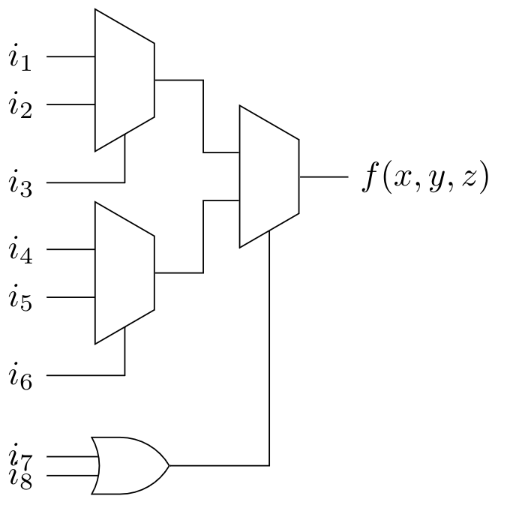
\includegraphics[scale=0.4]{./L04_Z08.png}
\end{center}
kolejno: $i_1=z, i_2 = y, i_3 = y, i_4 = y, i_5 = x, i_6 = z, i_7 = x, i_8 = y$\\
$i_1=z, i_2 = z, i_3 = z, i_4 = y, i_5 = x, i_6 = z, i_7 = y, i_8 = y$
ustalmy  że biorę multipleksery kolumnami (lewy górny to pierwszy, lewy dolny to drugi, prawy to trzeci)\\
lewy górny multiplekser to: $y+\bar{y}z$\\
lewy dolny multiplekser to: $\bar{z}y + zx$\\
prawy multiplekser to: $\neg(x + y)(y+\bar{y}z) + (x+y)(\bar{z}y + zx)=\bar{x}\bar{y}(y+\bar{y}z) + (x\bar{z}y + zx + \bar{z}y + xyz) = \bar{x}\bar{y}z + x\bar{z}y + zx + \bar{z}y + xyz = \bar{x}\bar{y}z + zx + \bar{z}y + xyz$  \\
lewy górny multiplekser to: $z$\\
lewy dolny multiplekser to: $\bar{z}y + zx$\\
prawy multiplekser to: $\bar{y}z + y(\bar{z}y + zx)= \bar{y}z + \bar{z}y + xyz =  \bar{y}z + \bar{z}y + xz$ \\


\section{Udowodnij o i-tym kodzie Graya, że $G(i) = i \oplus (i \gg 1)$.}

Możemy to zrobić dowodem indukcyjnym, podstawa indukcji:\\
\\
Krok indukcyjny:
To co będziemy robili to doklejali na początku kolejną liczbę. Rozpatrzymy na 2 przypadki:\\
1. doklejamy 0\\
	$G(0w) = 0(w \oplus (w \gg 1)= (0w \oplus (0w \gg 1)$\\
	zgodnie z definicją, zmieni się wyłącznie 1 bit.
2. doklejamy 1\\
	$G(1w) = 1(w \oplus (w \gg 1)= 1(\bar w \oplus \neg(w \gg 1) = 1(\bar w \oplus (1\bar w \gg 1)$\
%x(\bar y + 0\bar{z} +  z) + \bar{x}(\bar y + \bar z)=x(z(+\bar{z}\bar{y})) + \bar{x}(\bar z + z\bar y) = xz + x\bar{y}\bar{z} + \bar{x}\bar{z} + \bar{x}z\bar{y}
\end{document}